\section{Introducción.}
Los mercados hacen bien muchas cosas, pero no lo hacen todo bien, es así que en una economía de mercado, la interacción de la oferta y demanda es la que determina la cantidad y precio de equilibrio de los bienes y servicios transados. Asimismo, el mercado se encarga de la distribución de la renta a través de la posesión de los factores productivos (capital, trabajo, etc.) \\

Pero la competencia perfecta y las excelencias derivadas de este mercado como su pretendida eficiencia económica sólo se dan cuando se cumplen un conjunto de condiciones muy restrictivas que podemos calificar como de ideales, es decir, que la existencia de mercados 100\% eficientes es una construcción teórica que permite analizar los modelos económicos pero que difícilmente se da en la vida real debido a la existencia de algunos \textbf{fallos del mercado.}\\

Conocemos, por los \textit{"principios de la economía"} estudiados en el capitulo I, que \textit{"los mercados normalmente son un buen mecanismos para organizar la actividad económica"} (6º principio.) pero también sabemos que \textit{"el gobierno puede mejorar en algunas ocasiones los resultados del mercado" (8º principio).} Es así que ante la existencia de estos fallos del mercado es conveniente la intervención del gobierno a través de políticas gubernamentales específicas.\\

Una economía de mercado no siempre puede garantizar la distribución equitativa de los beneficios de la prosperidad económica, y ante un escenario que presenta inequidades, la intervención del gobierno se constituye en un mecanismo que permite lograr una distribución más equitativa del bienestar económico, pero para que el gobierno desarrolle determinadas acciones o políticas es fundamental conocer la realidad donde se va intervenir y esto se logra a través del manejo y conocimientos de las variables económicas y sociales de un determinado territorio.   
\begin{scaja}
	\paragraph{¿Por qué el Gobierno interviene la economía?}
	Una de las razones por las cuales necesitamos al gobierno es porque las economías de mercado necesitan instituciones que hagan
	valer los derechos de propiedad de las personas para que éstas puedan ejercer propiedad y control sobre los recursos escasos. Pero también necesitamos al gobierno para promover la eficiencia y la equidad en la economía ya que la mayoría de las medidas económicas aspiran a generar mayor crecimiento económico y mayor bienestar a través de una mejor redistribución de la riqueza.
\end{scaja}

\begin{definicion}[\textcolor[rgb]{0,0,0.55}{Fallos del mercado:}]
{\small 	Es una situación que se produce cuando el mercado, por si sólo, no es capaz de asignar los recursos de forma eficiente.}
\end{definicion}

\begin{definicion}[\textcolor[rgb]{0,0,0.55}{Estado:}]
	{\small Forma de organización política, dotada de poder soberano e independiente, que integra la población e instituciones de un territorio.}
\end{definicion}

\begin{definicion}[\textcolor[rgb]{0,0,0.55}{Gobierno:}]
	{\small Órgano superior del poder ejecutivo de un Estado o de una comunidad política, por tanto, son las autoridades que dirigen, controlan y administran las instituciones del Estado.}
\end{definicion}

\subsection{{\large Los fallos de mercado.}}
La existencia de fallos de mercado se puede deber a la presencia de alguno de los tres hechos siguientes: \textbf{competencia imperfecta, externalidades e información imperfecta.}\\

\subsubsection{\textcolor[rgb]{0,0,0.55}{\underline{{\normalsize Competencia Imperfecta:}}}}
Una posible causa de una falla de mercado se relaciona con el \textbf{poder de mercado} que tienen las empresas, esto es,
capacidad para influir sobre los precios que tiene y como a través de este poder se impide que exista un mercado eficiente en la economía.\\

El poder de mercado deriva en mercados no competitivos, entendido como son aquellos mercados en los que el productor o productores son lo suficientemente grandes como para tener un efecto notable sobre el precio. En los mercados de competencia imperfecta, el precio no se acepta como un dato ajeno, sino que los oferentes intervienen activamente en su determinación.\\

Las causas de imperfección en los mercados son los factores que suele impedir que se incorporen un mayor número de empresas en un mercado determinado y estas causas son principalmente dos:
\begin{itemize}
	\item Los costos de producción.
	\item Las barreras a la entrada de nuevos competidores en una industria 
\end{itemize}

\paragraph{{\normalsize Costos de Producción.}}
La estructura de costos y el nivel tecnológico son los factores determinantes del número de empresas que puede soportar una
industria o un mercado específico y las dimensiones que éstas pueden tener, por tanto, aquellos que puedan producir bienes y servicios a un menor costo tienen mayores posibilidades de incrementar su poder de mercado y por medio de estos limitar la cantidad de nuevos oferentes en una determinada industria o mercado. 

\begin{definicion}[\textcolor[rgb]{0,0,0.55}{Costos de Producción:}]
	Es el conjunto de gastos que son necesarios para producir bienes o servicios
\end{definicion}

\paragraph{{\normalsize Barreras de Entrada.}}
Las barreras de entrada a un mercado son obstáculos de diversos tipos que complican o dificultan el ingreso a un mercado de empresas, marcas o productos nuevos. Estas barreras representan un aspecto fundamental en la determinación de la estructura del mercado, ya que afectan sustancialmente el número de empresas, la concentración, la amenaza de entrada y el nivel de competencia de una industria. \\

Las principales barreras de entrada que enfrenta un potencia competidor las podemos clasificar en tres categorías: las restricciones legales, restricciones naturales y restricciones estratégicas.

\begin{itemize}
	\item \textbf{Barreras Legales:} Tienen su origen en la normativa y corresponden a aquéllas con las cuales, por algún cuerpo legal, se impide, o al menos se encarece, la entrada de nuevas empresas en una industria.
	\item \textbf{Barreras Económicas:} Están ligadas a la inversión necesaria para la entrada en el mercado de nuevos competidores, por ejemplo el gasto en publicidad enfocada a dar a conocer la nueva empresa y sus productos o la parte de inversión dedicada al desarrollo y la innovación tecnológica necesarios en gran número de sectores que permitan superar las barreras económicas ligadas a costos, precios o diferenciación de productos; Entre las principales barreras económicas podemos mencionar:
	\begin{itemize}
		\item \textbf{Economías a escala:} que relaciona los costos con la producción, existe economía de escala cuando el costo medio decrece con el nivel de producción. Es decir, cada unidad adicional que produce la empresa (constituida en determinado mercado) disminuye su costo unitario. 
		\item \textbf{Diferenciación de producto:} la diferenciación ocurre cuando las empresas ya establecidas tienen prestigio de marca o una cartera de clientes establecida.
		\item \textbf{Los precios:} Se pueden constituir en una barrera de entrada, si pensamos que 
		el caso de 	una empresa establecida fija los precios lo suficientemente bajos de manera que los potenciales entrantes
		se sientan desalentados de ingresar a la industria o mercado específico.
	\end{itemize}

Estas barreras de entrada, entendidas como los factores que limitan la entrada de nuevas empresas en una industria, de forma que, cuando las barreras de entrada son altas, la industria tendrá pocas empresas y escasas presiones para competir.  

\end{itemize}

\paragraph{{\normalsize Mercados de Competencia Imperfecta.}}
En función del número, del tamaño de los oferentes, del grado de concentración entre las empresas concurrentes y de la homogeneidad o heterogeneidad de los productos, podemos clasificar  los mercados de competencia imperfecta en tres categorías diferentes:
\begin{itemize}
	\item \textbf{El monopolio:} es el caso extremo de la competencia	imperfecta y se caracteriza porque hay un único vendedor
	que controla la industria.
	\item \textbf{El oligopolio:} este mercado se caracteriza porque hay pocos vendedores, de forma que cada empresa 
	puede influir en el precio de mercado y en la conducta 	de sus competidores.\\
\end{itemize}

\subsubsection{\textcolor[rgb]{0,0,0.55}{\underline{{\normalsize Externalidades:}}}}

Las externalidades se definen como decisiones de consumo, producción e inversión que toman los individuos, los hogares y las empresas y que afectan a terceros que no participan directamente los procesos antes referidos. Una externalidad surge cuando una persona se dedica a una actividad que influye en el bienestar de un tercero al que no se le paga ni se le compensa por dicho efecto.\\

Ante la presencia de externalidades, el intere?s de la sociedad en el resultado del mercado va ma?s alla? del bienestar de los compradores y vendedores que participan en el mercado, por tanto, la inclusión del bienestar de terceros que resultan afectados directa o indirectamente es por las acciones de compradores o vendedores es de mayor que el bienestar de estos último.\\

Si el impacto sobre el tercero es negativo, se conoce como externalidad negativa. Si le beneficia, se llama externalidad positiva:

\begin{itemize}
	\item     \textbf{Externalidad negativa:} Surge cuando no se asumen todos los costos de un efecto negativo. Hablamos de externalidades negativas cuando, por ejemplo, una empresa contamina su entorno o cuando una persona arroja basura a la calle. En estos dos casos, se genera un costo social, ya que es toda la sociedad por igual la que sufre las consecuencias de sus acciones y el precio de mercado no recoge este costo.
	\item \textbf{Externalidad positiva:} Surge de un efecto positivo que no se reporta como beneficio. Un ejemplo de externalidad positiva que podemos mencionar es la investigación científica, de la cual se beneficia la sociedad en general. Otro ejemplo sería la utilización de energías renovables, del que se beneficia la sociedad porque la persona o empresa que las utiliza no está contaminando. En estos casos, los precios de mercado no recogen los beneficios reales.
\end{itemize}

Entonces, cuando una \textbf{acción privada} tiene efectos colaterales o externos que afectan a otras personas de manera importante existe un problema de externalidades. Estos efectos externos crean una divergencia entre los costos y valoraciones privadas y sociales. Dado que los efectos externos no se reflejan en los precios de mercado, éstos facilitan informaciones que impiden alcanzar la eficiencia económica.

\begin{figure}[h]
	\centering
	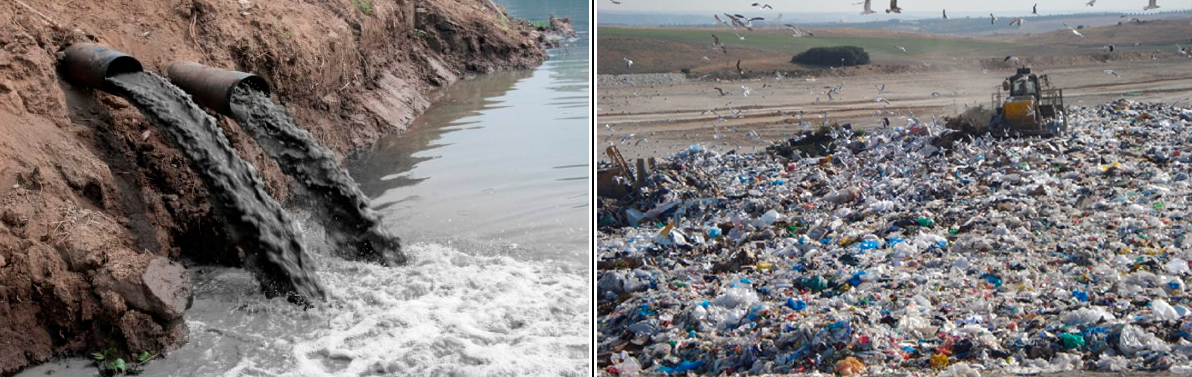
\includegraphics[width=0.7\linewidth]{images/contamina}
	\caption[Externalidades Negativas]{La contaminación como externalidad negativa (efecto de la producción y el consumo)}
	\label{fig:contamina}
\end{figure}

Buena parte de las externalidades negativas se deben a la contaminación. Las ciudades contaminan los ríos, los lagos y los mares con sus vertidos y las empresas con los suyos. Los automóviles, las calefacciones y las industrias contaminan la atmósfera. Estas externalidades crean ineficiencias.

\begin{definicion}[\textcolor[rgb]{0,0,0.55}{Externalidad}]
	El efecto no compensado de las acciones de una persona sobre el bienestar de un tercero.
\end{definicion}

\begin{ejemplos}
	Las externalidades se presentan en diferentes formas, al igual que las políticas que se formulan para corregir las fallas del mercado. He aquí algunos ejemplos:
	\begin{ejemplo}
		El tubo de escape de los automóviles es una externalidad negativa porque genera smog que otras personas tienen que respirar. Como resultado de esta externalidad, los conductores tienden a contaminar demasiado. El gobierno trata de resolver este problema estableciendo normas para las emisiones de los automo?viles, tambie?n podrian aplicar un impuestos a la gasolina para reducir la cantidad de personas que conducen vehi?culos automotores.
	\end{ejemplo}
	\begin{ejemplo}
	Los edificios históricos restaurados constituyen una externalidad positiva, porque las personas que pasan por donde se encuentran disfrutan de su belleza y el recuerdo de la historia que evocan. Los propietarios de los edificios no obtienen el beneficio total de la restauración y, en consecuencia, tienden a deshacerse muy rápido de los edificios viejos. Muchos gobiernos locales responden a este problema regulando la destrucción de edificios histo?ricos y ofreciendo exenciones de impuestos a los propietarios que los restauran.
    \end{ejemplo}

	\begin{ejemplo}
	Los perros que ladran crean una externalidad negativa, porque el ruido molesta a los vecinos. Los dueños de los perros no cubren el costo total del ruido y, por tanto, tienden a tomar pocas medidas precautorias que impidan que sus perros ladren. Para resolver este problema los gobiernos locales prohíben "alterar el orden pu?blico".
	\end{ejemplo}

	\begin{ejemplo}
	La investigacioón de nuevas tecnologi?as es una externalidad positiva porque crea conocimiento que otras personas pueden utilizar. Debido a que los investigadores no pueden captar los beneficios completos de sus inventos, tienden a destinar pocos recursos a la investigacio?n.
	\end{ejemplo}
En cada uno de estos casos, algún tomador de decisiones no considera los efectos externos de su comportamiento. En respuesta, el gobierno trata de influir en su comportamiento para proteger los intereses de terceros.
\end{ejemplos}

\paragraph{{\normalsize Instrumentos del Estado para combatir las externalidades.}}
Debido a que compradores y vendedores desatienden los efectos externos de sus acciones cuando deciden cuánto demandar u ofrecer, por tanto, el equilibrio del mercado no es eficiente cuando se presentan externalidades, es decir, el equilibrio es incapaz de maximizar el beneficio total para la sociedad.\\

Para luchar contra la ineficiencia derivada de las externalidades, los Estados suelen establecer "regulaciones sociales" a través de \textbf{controles directos}, o bien recurrir a \textbf{incentivos económicos}, es decir, "medidas basadas en el mercado".
\begin{itemize}
	\item \textbf{Regulaciones Sociales:} Para dar solución a una externalidad, el gobierno puede exigir o prohibir ciertas conductas mediante la aplicación de \textbf{\textcolor[rgb]{0,0.24,0.5}{"Controles Directos."}} Por ejemplo, es un delito verter sustancias químicas venenosas en el sistema de abastecimiento de agua. En este caso, los costos externos para la sociedad exceden	por mucho los beneficios para el que contamina. Por tanto, el gobierno instituye una	política de orden y control que prohíbe este tipo de actos.\\
	
	Los controles directos se constituyen en detalladas instrucciones sobre las acciones a tomar, la tecnología que se debe utilizar para controlar la contaminación y dónde se debe aplicar. Las leyes y normas o regulaciones ambientales son tipos de controles que establecen los gobiernos prohibiendo determinadas acciones o estableciendo procedimientos para minimizar los efectos negativos derivados de las actividades comerciales o de consumo, además de estipular las penalizaciones a pagar por los daños causados a otras personas.\\
	
	Pero este tipo de controles directos no dejan margen para aplicar nuevos métodos que permitan combatir las externalidades y la experiencia nos muestran que los resultados de la aplicación de dichos controles sueles se costos y derivan en la vulneración de las mismas.
	
	\item \textbf{Medidas Basadas en el Mercado:} Un segundo tipo de instrumentos para combatir la ineficiencia	provocada por las externalidades, y en particular la contaminación, son los que recurren a \textbf{\textcolor[rgb]{0,0.24,0.5}{"incentivos económicos"}} que proporciona el mercado. En este sentido son dos los tipos de soluciones empleadas: \textbf{los impuestos sobre emisiones} y los \textbf{permisos transferibles de contaminación.}\\
	
	\textbf{\textcolor[rgb]{0,0.24,0.5}{Impuesto sobre emisiones:}} Son un tipo de \textbf{impuesto correctivo} que tiene el propósito de inducir a los sujetos responsables de la externalidad ha tomar en cuenta el costo social que surge de una determinada actividad desarrollada por estos, es así que los impuestos sobre las emisiones obligan, por ejemplo, a las empresas a pagar un impuesto sobre su contaminación igual a la cantidad de daños externos ocasionados.\\
	
	En esencia, este tipo de impuestos asigna un precio al derecho a contaminar, por tanto, pretende internalizar la externalidad forzando a los sujetos contaminantes pague los costos sociales de sus actividades (producción y/o consumo).\\
	
	\textbf{\textcolor[rgb]{0,0.24,0.5}{Permisos transferibles para contaminar:}} Cuando se recurre a este método, en vez de obligarle a la empresa contaminante a pagar una determinada cantidad por unidad de contaminación y permitirle elegir el nivel de contaminación, las autoridades eligen el nivel o umbral máximo de contaminación total y determinan el número adecuado de permisos.\\
	
	Este método de actuar permite que las empresas contaminantes que pueden reducir sus emisiones de forma más barata lo hagan y vendan sus permisos a las	que necesitan más permisos para nuevas plantas o porque	no tienen mucho margen para reducir las emisiones y les	resulta más conveniente comprar permisos en lugar de instalar unos equipos caros contra la contaminación.\\
	
\end{itemize}


\subsubsection{\textcolor[rgb]{0,0,0.55}{\underline{{\normalsize Información Incompleta:}}}}
El tercer tipo de fallo del mercado, junto a la competencia
imperfecta y las externalidades, es la \textbf{información imperfecta.} La teoría de libre mercado supone que los compradores y los vendedores tienen total información sobre
los bienes y los servicios que compran y venden. Se supone que las empresas conocen perfectamente todos los aspectos técnicos necesarios para producir en su industria y que los consumidores conocen la calidad y los precios de los bienes que consumen. Por ejemplo, se supone que los consumidores saben qué automóviles se encuentran en buen estado y cuales no o cuál es la seguridad y la eficacia de los fármacos que toman. \\

La realidad es muy distinta de este mundo idealizado y lo relevante es saber en qué medida son perjudiciales las desviaciones respecto de la información perfecta. En algunos casos, la pérdida de eficiencia es escasa. Así, por ejemplo, apenas resultaremos perjudicados si compramos una pizza con una masa distinta de la de otra. En otros casos, la pérdida es grave. Entonces, \textit{los mercados normalmente suministran a los consumidores o a los productores una información imperfecta para la toma de decisiones.}\\

La realidad es muy distinta de este mundo idealizado ya que la información asimétrica es característica de muchas situaciones de la vida real. A menudo el vendedor de un producto conoce su calidad mejor que el comprador. Normalmente los trabajadores conocen sus propias cualificaciones y capacidades mejor que los empresarios, los directivos conocen mejor los costes de la empresa, la posición competitiva y las oportunidades de inversión que los propietarios o accionistas y los médicos suelen tener más información sobre las enfermedades que los pacientes.\\

Para analizar las implicaciones de la existencia de información imperfecta, empecemos por considerar qué ocurre cuando algunos tienen más información que otros, es decir, cuando hay \textbf{información asimétrica}, existirá \textcolor[rgb]{0,0.18,0.39}{información asimétrica cuando la información sobre la calidad y características de los bienes y servicios intercambiados o sobre las acciones o características de los agentes que influyen en aquéllas no está distribuida de forma simétrica entre los consumidores y los productores,} por tanto, la existencia asimetrías de información puede afectar el nivel de precios en los mercados como consecuencia del uso indebido de la información privilegiada.\\

\subsection{{\large Las Funciones del Estado.}}

Tal como hemos señalado, las economías de mercado tienen imperfecciones que generan
males como la contaminación excesiva, el desempleo y diferencias de renta y riqueza que se consideran éticamente rechazables. Esto significa que las economías de mercado no se
ajustan totalmente al mundo idealizado de la mano invisible que funciona armoniosamente. Por estas razones, el Estado asume muchas tareas que tratan de paliar los fallos
del mecanismo del mercado.\\

El Estado interviene en la actividad económica procurando la eficiencia, la equidad, la estabilidad económica y el crecimiento y el bienestar. Este conjunto de actividades del Estado se engloban en tres grandes funciones que son:\\
\begin{itemize}
	\item Mejorar la eficiencia económica combatiendo los
	fallos del mercado.
	\item Estabilizar la economía y propiciar el crecimiento
	económico, mediante la política económica.
	\item Procurar la equidad mejorando la distribución de la
	renta.
\end{itemize}
El Estado contribuye a la asignación socialmente deseable de los recursos. En este sentido, el Estado interviene tratando de contribuir a corregir los fallos del
mercado analizados previamente (competencia imperfecta, las externalidades y la información imperfecta). En este sentido, el Estado interviene tratando de limitar el poder
de mercado de las empresas monopolísticas u oligopolísticas, luchando contra los efectos nocivos de las externalidades, especialmente la contaminación, proveyendo bienes públicos y tratando de suministrar información a los consumidores para que tomen decisiones
bien documentadas y así paliar los efectos de la información imperfecta.\\

\subsubsection{El Estado y la Actividad Económica:}

El Estado en la búsqueda de sus objetivos recurre a diferentes instrumentos que le permita cumplir sus funciones, es así que la Política Fiscal y la Política Monetaria son los principales instrumentos del Estado para intervenir en la actividad económica.\\

	\textbf{\textcolor[rgb]{0,0.24,0.5}{Política Fiscal:}}	\small Se entiende por política fiscal al \textbf{conjunto de medidas relativas al régimen tributario, gasto publico, endeudamiento interno externo del Estado, y a las operaciones y situación financiera de las entidades y organismos autónomos. } \\
	
	\textbf{\textcolor[rgb]{0,0.24,0.5}{Política Monetaria:}} \small Es el conjunto de acciones llevadas por el \textbf{Banco Central}, \textbf{cuyo fin es influir en el crecimiento económico mediante manejo de variables monetarias de la economía.} Variables como la inflación, emisión monetaria, funcionamiento del banco Central, regulación de bancos comerciales, tipo de interés, protección a reservas de oro y dólares.\\
	
	La política fiscal y monetaria tiene un abanico de instrumentos, pero son tres los instrumentos básicos que utiliza el Estado para influir en la actividad económica: los \textbf{impuestos}, los	\textbf{gastos} y la \textbf{regulación}.\\
	
	\begin{cajaejercicios1}[Impuestos]
		Los impuestos son un pago al Estado, y estos reducen la renta privada y el gasto privado y son fuente de recursos para el gasto público. \\
		
		El conjunto impuestos, esto es, el sistema tributario,	también sirve para reducir los incentivos para llevar a cabo determinadas actividades sujetas a impuestos,
		como contaminar o fumar, y fomentar otras que están	menos gravadas, como es comprar una vivienda, estudiar	o investigar, etc.\\
				
		Cuando el Estado establece los impuestos está decidiendo la manera en que van a obtenerse los recursos necesarios de los hogares y de las empresas para darle un fin público, es decir, el Estado para hacer frente a los gastos públicos, esto es, a todos	los programas, proyectos y actividades llevadas a cabo por el mismo,
		el Estado establece una serie de impuestos y lo que falta lo obtiene mediante crédito.\\
		
	\end{cajaejercicios1}

	\begin{cajaejercicios1}[Gastos]
		El gasto público es la cantidad de recursos financieros, materiales y humanos que el sector público representado por el gobierno emplea para el cumplimiento de sus funciones, este conjunto de erogaciones que realiza el Estado esta orientado a la producción bienes y servicios públicos en un periodo determinado.\\
		
		El gasto público comprende desde las compras de bienes	y servicios por parte del sector público a los sueldos de los	funcionarios públicos, la Seguridad Social y otras transferencias, y los intereses. De igual forma las inversiones públicas forman parte del gasto público total reflejados en programas y proyectos de inversión pública.\\
		
		Desde la perspectiva de gestión del gasto público se pueden identificar tres objetivos principales:
		\begin{itemize}
			\item Lograr estabilidad económica y la disciplina fiscal.
			\item Alcanzar una adecuada distribución social de los recursos.
			\item Promover la eficiencia a través de gasto público, mediante la corrección de fallas de mercado
		\end{itemize}
	\end{cajaejercicios1}
	Estos objetivos tienen la finalidad de generar mayores niveles de crecimiento y desarrollo económico y por medio de estos bienestar para su población.\\
	
	\begin{cajaejercicios1}[Regulación]
		La regulación, es el control por parte del Estado de la actividad económica, estas regulaciones lleva a los individuos y empresas a realizar determinadas actividades o abstenerse de realizarlas.\\
		
		Desde una perspectiva general la regulación es de dos tipos: económica y social. 
		\begin{itemize}
			\item La \textbf{regulación económica} se refiere al control de los precios, la producción, las condiciones de entrada y salida del mercado y la calidad de los	productos y servicios de una determinada industria.\\
			
			\begin{definicion}[\textcolor[rgb]{0,0,0.55}{Regulación Económica:}]
				La regulación económica consiste en las normas destinadas a controlar las decisiones de las empresas relacionadas con los precios, las ventas
				o la producción.
			\end{definicion}

			
			\item La \textbf{regulación social} es la que se emplea para proteger
			el medio ambiente, la salud y la seguridad de los trabaja-
			dores y de los consumidores, y se encamina a tratar de
			corregir los efectos secundarios o externalidades de la
			actividad económica.
			 
		\end{itemize}
	\end{cajaejercicios1}
\subsection{{\large Variables Socioeconómicas.}}
Si la finalidad del Gasto Público, como política fiscal, es el de generar mayores niveles de crecimiento y desarrollo económico y por medio de estos bienestar para su población, es importante poder precisar que debemos entender por Crecimiento, Desarrollo o Subdesarrollo y Bienestar y como el analizar estas condiciones a través de variables socioeconómicas permitirán desarrollar diagnósticos mas precisos y orientar las decisiones de gasto público.\\

% Define box and box title style
\tikzstyle{mybox} = [draw=azul1!90, fill=yellow!15, very thick,
rectangle, rounded corners, inner sep=10pt, inner ysep=10pt]
\tikzstyle{fancytitle} =[fill=azul1!90, text=white]

\begin{tikzpicture}
\node [mybox] (box){%
	\begin{minipage}{0.95\textwidth}
	El crecimiento económico es definido como la capacidad de una economía para producir cada vez más bienes y servicios, por tanto, es el aumento del producto e ingreso.
	\end{minipage}
};
\node[fancytitle, right=10pt] at (box.north west) {\textbf{Crecimiento Económico}};
%\node[fancytitle, rounded corners] at (box.east) {$\clubsuit$};
\end{tikzpicture}
\\
%%%%%%%%%%%%%%%%%%%%%%%%%%%%%%%%%%%%

\tikzstyle{mybox} = [draw=miverde, fill=yellow!15, very thick,
rectangle, rounded corners, inner sep=10pt, inner ysep=10pt]
\tikzstyle{fancytitle} =[fill=miverde, text=white]

\begin{tikzpicture}
\node [mybox] (box){%
	\begin{minipage}{0.95\textwidth}
	El desarrollo económico puede definirse genéricamente como crecimiento
	sostenible desde tres puntos de vista: económico, social y medioambiental,
	por tanto, una mejora en el desarrollo económico se ve reflejado en el
	incremento del bienestar material de la población.
	\end{minipage}
};
\node[fancytitle, right=10pt] at (box.north west) {\textbf{Desarrollo Económico}};
%\node[fancytitle, rounded corners] at (box.east) {$\clubsuit$};
\end{tikzpicture}
\\
%%%%%%%%%%%%%%%%%%%%%%%%%%%%%%%%%%%%

\tikzstyle{mybox} = [draw=rojo1, fill=yellow!15, very thick,
rectangle, rounded corners, inner sep=10pt, inner ysep=10pt]
\tikzstyle{fancytitle} =[fill=rojo1, text=white]

\begin{tikzpicture}
\node [mybox] (box){%
	\begin{minipage}{0.95\textwidth}
	Es la situación de un país o región que no alcanza determinados niveles de crecimiento económicos, sociales y mediambientales.
	\end{minipage}
};
\node[fancytitle, right=10pt] at (box.north west) {\textbf{Subdesarrollo}};
%\node[fancytitle, rounded corners] at (box.east) {$\clubsuit$};
\end{tikzpicture}

\begin{scaja}
		\textbf{El subdesarrollo es una estructura productiva atrasada en comparación con otros países}, las condiciones de vida de la población son limitadas, se tiene dependencia con el mercado internacional, 	desigualdad económica, no se tienen bienes de capital para la inversión en rubros necesarios para	el país, los sectores industriales son insuficientes o atrasados, hay baja productividad, bajos salarios y 	competencia con productos importados, entre otros factores.
\end{scaja}

Si las condiciones de vida de la población son limitada, es obligación del gobierno de dirigir sus esfuerzos de política económica a generar las condiciones de desarrollo, por tanto de bienestar para su población, pero la pregunta que surge ante esta situación es: \textbf{¿Cómo podemos medir el nivel de desarrollo de un país, región o localidad?}, y así enfocar los esfuerzo en las situaciones más problemáticas.\\

Una aproximación a la caracterización del mundo desarrollado y subdesarrollado
o en vías de desarrollo se puede obtener analizando los indicadores
socioeconómicos (\textcolor[rgb]{0,0.25,0.25}{variables socioeconómicas}) y comparando sus diferentes valores.
\\
%%%%%%%%%%%%%%%%%%%%%%%%%%%%%%%%%%%%

\tikzstyle{mybox} = [draw=rojo1, fill=red!15, very thick,
rectangle, rounded corners, inner sep=10pt, inner ysep=10pt]
\tikzstyle{fancytitle} =[fill=rojo1, text=white]

\begin{tikzpicture}
\node [mybox] (box){%
	\begin{minipage}{0.95\textwidth}
	De igual forma, si como estudiantes o el su futuro campo laboral, deben desarrollar proyectos de grado o proyectos de inversión, estos deben contar con un diagnostico base, que supone entre otras tareas, analizar las variables socioeconómicas más relevantes de acuerdo a la naturaleza del trabajo de investigación.
	\end{minipage}
};
%\node[fancytitle, right=10pt] at (box.north west) {\textbf{Subdesarrollo}};
%\node[fancytitle, rounded corners] at (box.east) {$\clubsuit$};
\end{tikzpicture}


%\subsection{{\large Los .}}
